\documentclass[11pt,a4paper,twoside, openany]{book}



%%---------- Packages ---------------------------------------------------------
\usepackage[a4paper,includeheadfoot,margin=2.50cm]{geometry}
\usepackage[utf8]{inputenc}  % Accenten gebruiken in tekst (vb. é ipv \'e)
\usepackage{amsfonts}        % AMS math packages: extra wiskundige symbolen enz
\usepackage{amsmath}        
\usepackage{amssymb}
\usepackage[dutch]{babel}    % Taalinstellingen: woordsplitsingen,
                             % commando's voor speciale karakters
\usepackage{graphicx}        % Invoegen van tekeningen
	\graphicspath{{./img/}}
\usepackage{subcaption}
\usepackage{hyperref}        % PDF krijgt klikbare links & verwijzingen in de inhoudstafel
\usepackage{pdfpages}        % Laat het importeren van PDFs toe
\usepackage[acronym,toc]{glossaries} % Woordenschat
%	\hypersetup{
%		colorlinks,
%		citecolor=black,
%		filecolor=black,
%		linkcolor=black,
%		urlcolor=black
%	}
\usepackage{parskip} % Verwijdert indentatie van de paragrafen
\usepackage{lipsum}  % Lorem ipsum vultekst
\usepackage[numbers]{natbib}
\usepackage{ulem}
\usepackage[nottoc]{tocbibind} 

\newcommand{\todo}[1]{\color{red}\_ToDo: #1 \color{black}}
\newcommand{\remark}[1]{\color{purple}\_Opmerking: #1 \color{black}}
\newcommand{\source}[1]{\caption*{Bron: {#1}}}

\newacronym{hmm}{HMM}{Hidden Markov Model}
\makeglossaries

\pagestyle{headings}

\begin{document}
	
	
	
%	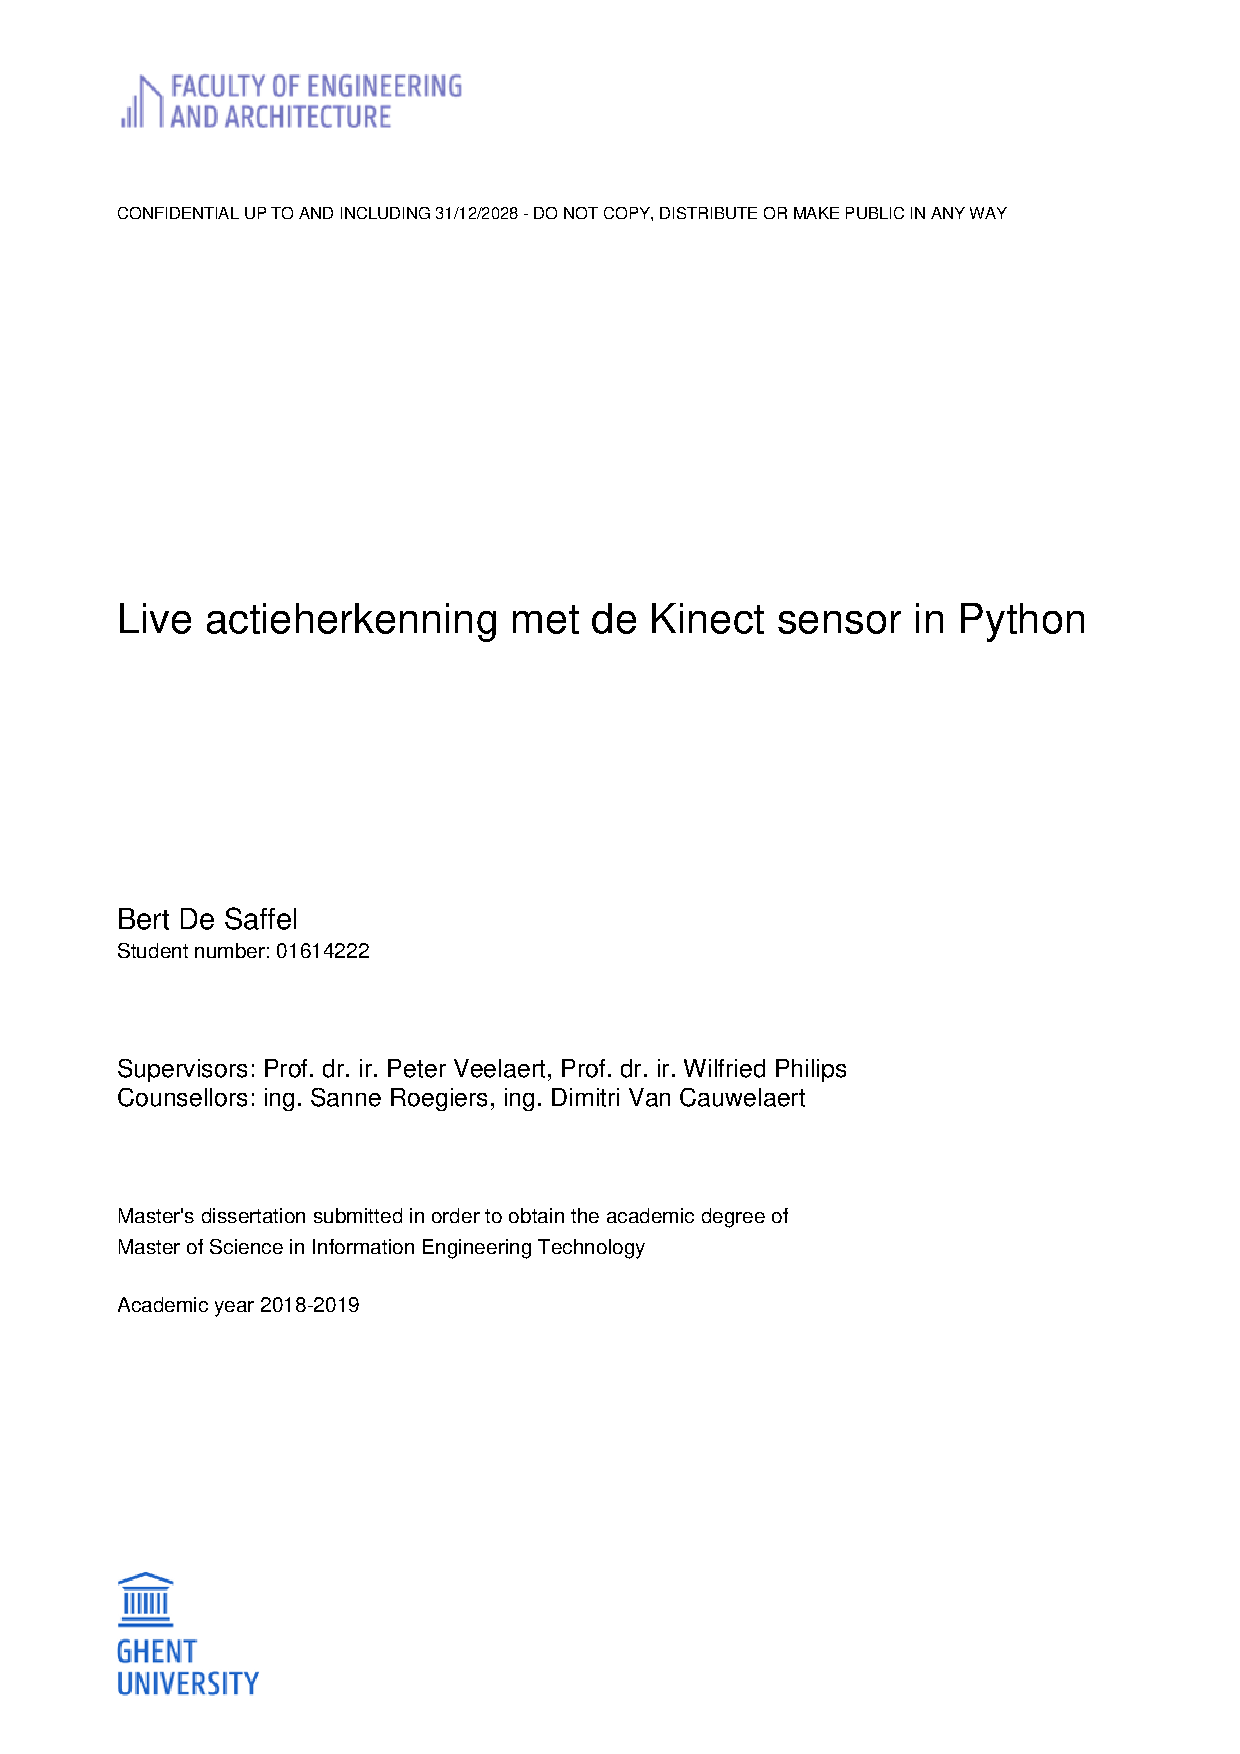
\includepdf{voorblad.pdf} 
%	\newpage\thispagestyle{empty}\mbox{}
%	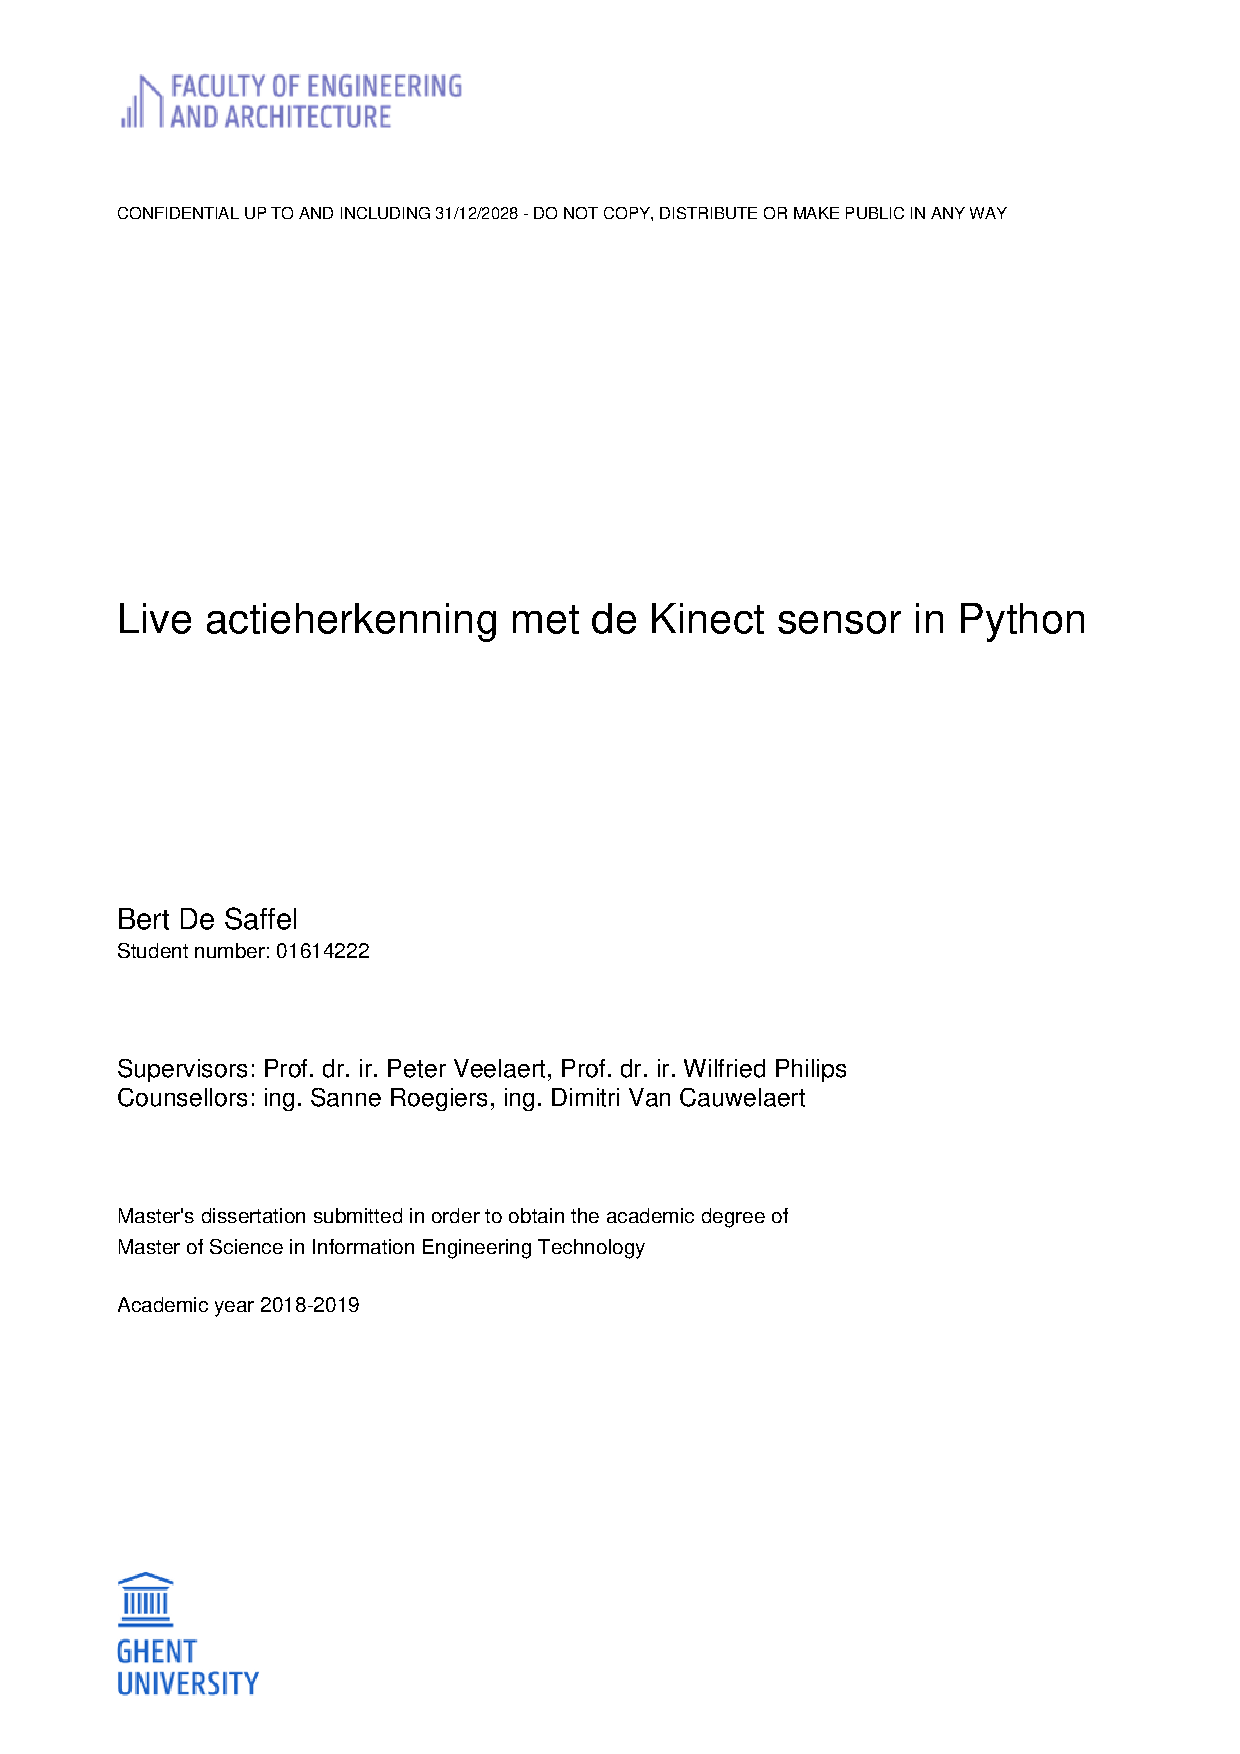
\includepdf{voorblad.pdf} 
	
%	\chapter*{Voorwoord}
\label{ch:Voorwoord}


%	\renewcommand{\abstractname}{Abstract}
\begin{abstract}
	
\end{abstract}
	%\todo{EXTENDED ABSTRACT}
	
	\pagenumbering{gobble} % voorkomen dat table of contents ook een paginanummer krijgt
	\tableofcontents
	
	
	\chapter{Inleiding}
\section{Compilers}
Voorbeelden van functies die een statische compiler moet bevatten:
	\begin{itemize}
		\item Broncode omzetten in uitvoerbare fouten:
		\begin{itemize}
			\item met dezelfde semantiek
			\item zo snel mogelijk
			\item en/of zo compact, debugbaar, portable, veilig, ... mogelijk
			\item en linkbaar.
		\end{itemize}
		\item Syntaxfouten moeten herkent worden.
	\end{itemize}

\section{Basiswerking compilers}
\begin{figure}[h]
	\centering
	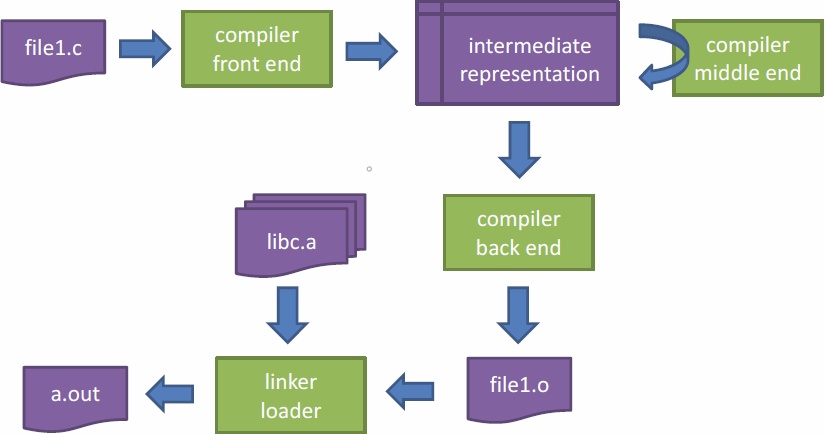
\includegraphics[width=0.5\textwidth]{basiswerking_compilers}
	\caption{De basiswerking van een compiler.} 
	\label{fig:basiswerking_compilers}
\end{figure}
Op figuur \ref{fig:basiswerking_compilers} is de vereenvoudigde basiswerking van een compiler te zien. Een \textbf{C} bestand wordt eerst door de \uline{compiler front end} gestuurd, die het bestand zal omvormen tot een intermediaire representatie. Deze representatie wordt dan door de \uline{compiler back end} gestuurd om zo assembly of objectcode te genereren. De \uline{linker loader} zal deze objectcode samenvoegen met eventuele andere libraries om zo een uitvoerbaar programma te hebben. 

\QA{Waarom wordt de front end en back end opgesplitst?}
{Op die manier is de compiler modulair: Enerzijds moet bij een andere programmeertaal enkel de front end aangepast worden en anderzijds moet bij het wijzigen van de architectuur (de onderliggende processor) enkel de back end aangepast worden.}


\section{Abstract Syntax Tree}
De eerste stap van elke compiler is het omvormen van de broncode naar een \textbf{Abstract Syntax Tree (AST)}. Veronderstel volgende code, en de daarbijhorende AST die te zien zijn op figuur \ref{fig:abstract_syntax_tree}. Elke knoop van een AST stelt een bepaalde geldige operatie voor, die afhankelijk is van de gekozen programmeertaal.
\begin{figure}[h]
	\centering
	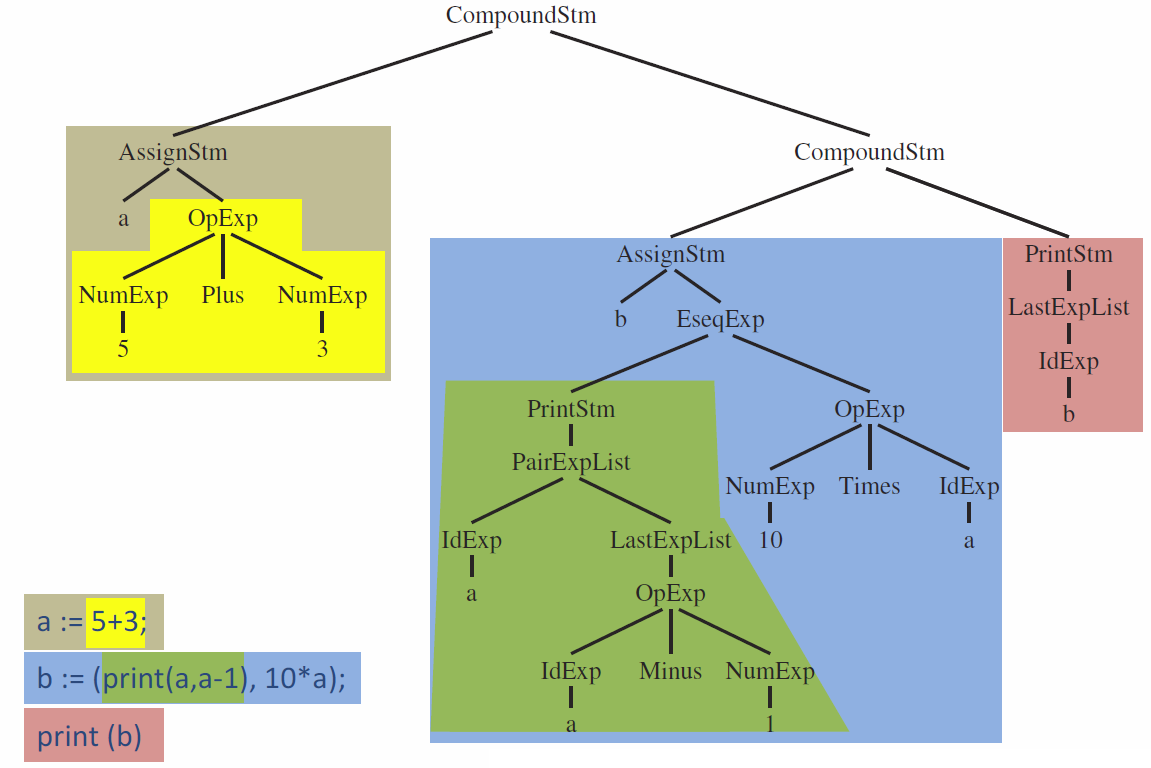
\includegraphics[width=0.8\textwidth]{abstract_syntax_tree}
	\caption{De boomvoorstelling van een eenvoudig, lusloos programma. De gekleurde deelbomen komen overeen met de gekleurde segmenten in de code zelf. Als toekenningsoperator wordt er gekozen voor $:=$ dat vanaf nu als één geheel moet beschouwd worden.}
	\label{fig:abstract_syntax_tree}
\end{figure}

\subsection{Contextvrije grammatica's}
Om een AST op te stellen moet de notie van \textbf{tokens} ingevoerd worden. Een token is eenvoudig gezien een bepaald symbool dat een betekenis heeft. De tokens van de code uit figuur \ref{fig:abstract_syntax_tree} zijn te zien in tabel \ref{table:tokens}
\begin{table}[h]
	\centering
	\begin{tabular}{l | l | l}
		symbolen(ascii) & token & waarde \\
		\hline
		a & id & string a \\
		:= & := & \\
		5 & num & integer 5 \\
		+ & + & \\
		3 & num & integer 3 \\
		; & ; & \\
		b & id & string b \\
		( & ( & \\
		print & print & \\
		- & - & \\
		* & * & \\
		  & whitespace & \\
	\end{tabular}
	\caption{De tokens die voorkomen uit het programma van figuur \ref{fig:abstract_syntax_tree}}
	\label{table:tokens}
\end{table}
Uit de theorie van de generatieve grammatica's weten we dat er zowel terminale als niet-terminale tokens bestaan:
\begin{itemize}
	\item \textbf{Terminale tokens} zijn symbolen die een blad voorstellen in de AST. Deze tokens hebben als eigenschap dat ze geen verdere tokens kunnen genereren en vormen dan ook het alfabet van het programma.
	\item \textbf{Niet-terminale tokens}, kortweg niet-terminalen genoemd, zijn de regels die de taal definiëren en zijn de niet-bladeren van de AST. Niet-terminalen hebben als eigenschap dat ze letters van het alfabet kunnen genereren.
\end{itemize}
Op figuur \ref{fig:contextvrije_grammatica} zijn een aantal terminalen en niet-terminalen te zien. De niet-terminale token \textit{CompoundStm} bestaat bijvoorbeeld uit twee \textit{Stm} tokens, gescheiden door een punt komma. Deze twee \textit{Stm} tokens kunnen in deze vereenvoudigde programmeertaal enkel een \textit{AssignStm} of \textit{PrintStm} zijn. Bij \textit{AssignStm} wordt er een terminale token verwacht in de vorm van een variabele identifier, gevolgd door de toekenningsoperator en een \textit{Exp} token. Enkel deze \textit{Exp} kan nog vier vormen aanneemen: \textit{IdExp}, \textit{NumExp}, enz...
{
\begin{figure}[h]
	\definecolor{cvred}{RGB}{215,149,146}
	\definecolor{cvblue}{RGB}{145,202,219}
	\centering
	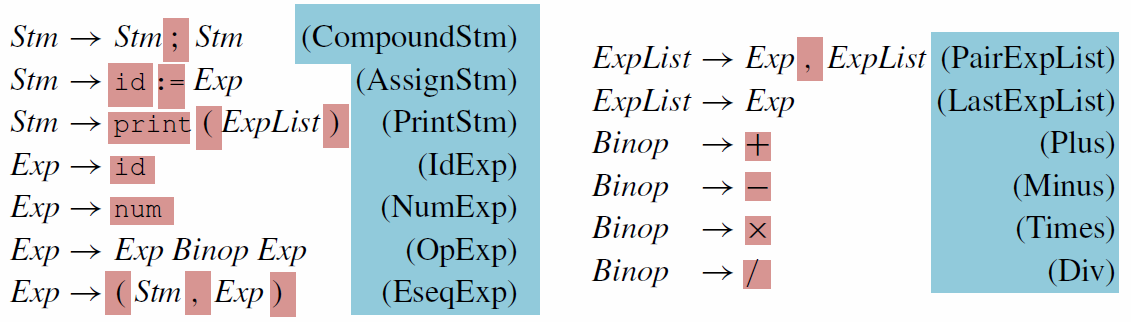
\includegraphics[width=0.8\textwidth]{contextvrije_grammatica}
	\caption{De rood omkaderde symbolen zijn {\color{cvred} terminalen} terwijl de blauw omkaderde {\color{cvblue}niet-terminalen} zijn.} 
	\label{fig:contextvrije_grammatica}
\end{figure}
}
Dit wordt uitgewerkt voor de eerste toekenningsoperatie uit figuur \ref{fig:abstract_syntax_tree} en is te zien op figuur \ref{fig:contextvrije_grammatica_voorbeeld}.
\begin{figure}[h]
	\centering
	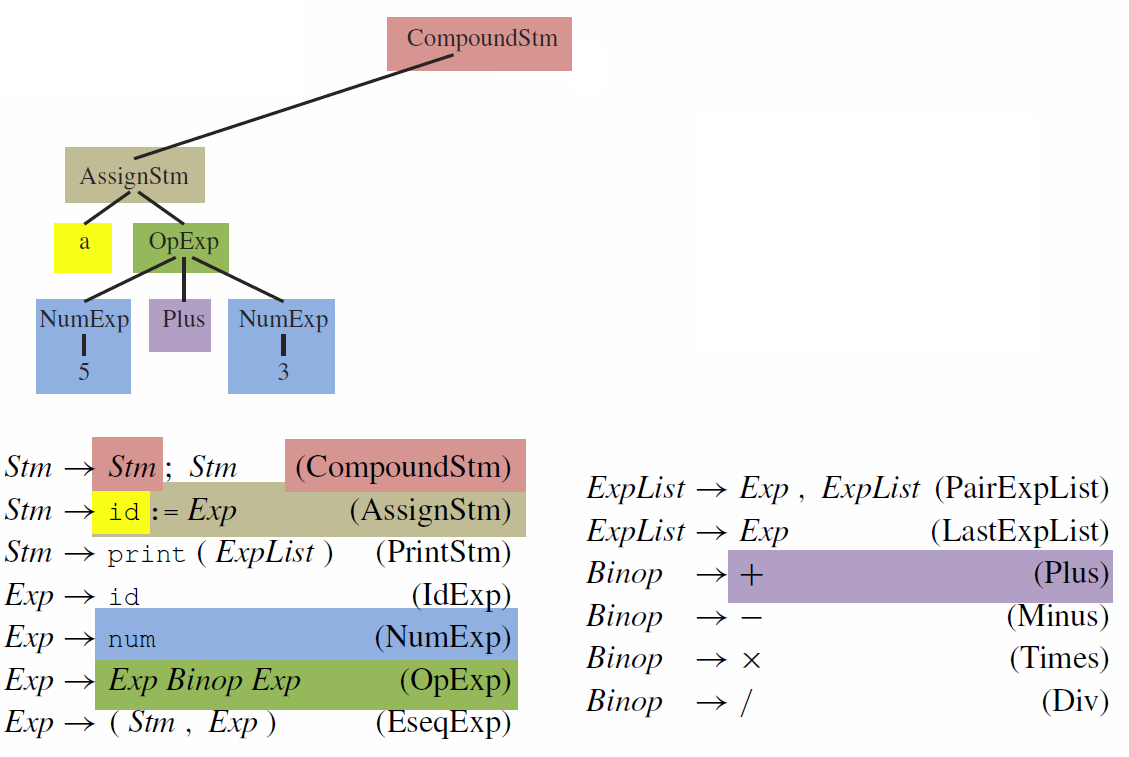
\includegraphics[width=0.8\textwidth]{contextvrije_grammatica_voorbeeld}
	\caption{Illustratie van contextvrije grammatica op de eerste toekenningsoperatie uit figuur \ref{fig:abstract_syntax_tree}.} 
	\label{fig:contextvrije_grammatica_voorbeeld}
\end{figure}

\subsection{Opbouw AST}
Een AST kan nu \textbf{bottom-up} opgemaakt worden door volgende procedure uit te voeren:
\begin{enumerate}
	\item Voor elke mogelijke knoop moet er een struct gemaakt worden zoals bijvoorbeeld:
	
	$$\texttt{A\_stm\_} \qquad \texttt{A\_exp\_} \qquad \texttt{A\_expList\_}$$
	
	\item Elke struct moet bestaan uit
	\begin{itemize}
		\item een enum voor het precieze token te bepalen,
		\item een union voor de verschillende combinaties van tokens in het rechter lid en,
		\item pointers naar kindknopen.
	\end{itemize}
	Dit wordt geïllustreerd in code \ref{lst:vb_struct_AST}.
	\begin{lstlisting}[caption={Voorbeeld van een struct voor een AST.},label={lst:vb_struct_AST}, captionpos=b]
typedef char * string;
typedef struct A_stm_ * A_stm;
typedef struct A_exp_ * A_exp;
typedef struct A_expList_ * A_expList;

struct A_stm_ {
	enum {A_compoundStm, A_assignStm, A_printStm} kind;
	union {
		struct {A_stm stm1, stm2;} compound;
		struct {string id; A_exp exp;} assign;
		struct {A_expList exps;} print;
	} u;
};
	\end{lstlisting}
	\item In de constructor worden de knopen aangemaakt, zoals te zien in code \ref{lst:vb_constructor_AST}.
	\begin{lstlisting}[caption={Voorbeeld van een constructor voor een AST.},label={lst:vb_constructor_AST}, captionpos=b]
A_stm A_CompoundStm(A_stm stm1, A_stm stm2){
	A_stm s = malloc(sizeof(*s));
	s->kind = A_compoundStm;
	s->u.compound.stm1 = stm1;
	s->u.compound.stm2 = stm2;
	return s;
}
	\end{lstlisting}
	
Op deze manier zou de boom uit figuur \ref{fig:abstract_syntax_tree} hardgecodeerd kunnen worden, wat natuurlijk geen goede manier is. Het is de taak van een \uline{lexer} en \uline{parser} om de constructie van een AST te automatiseren, die respectievelijk in hoofdstuk \ref{ch:lexicale_analyse} en \ref{ch:parsing} behandelt worden.

\subsection{Interpreter}
Uit een AST kan een eenvoudige interpreter geschreven worden. Dit stuk is informatief, en wordt niet gevraagd op het examen.
\begin{itemize}
	\item Door de boom postorder diepte-eerst te overlopen, wordt de boom in de juiste manier behandelt.
	\item Het bijhouden van de waarden van variabelen kan via een gelinkte lijst:
	\begin{lstlisting}
typedef struct table * Table_;
struct table {string id; int value; Table_ tail;};
Table_ Table(string id; int value; Table_ tail) {
	Table_ t = malloc(sizeof(*t));
	t->id = id;
	t->value = value;
	t->tail = tail;
	return t;
}
	\end{lstlisting}
	\item Stel nu dat dit de eerste drie regels van een programma zijn:
	\begin{lstlisting}
a := 2;
b := 3;
a := 3;
	\end{lstlisting}
	\item Voor de eerste toekenning bevat de gelinkte lijst slechts één knoop met als sleutel \textit{a} en waarde \textit{2}. 
	\item Bij de tweede toekenning wordt de originele gelinkte lijst meegegeven via de variabele \textit{tail}. Na deze constructor zal de gelinkte lijst twee knopen bevatten.
	\item Na deze constructor bevat de gelinkte lijst drie knopen. Merk op dat er twee knopen zijn met sleutel \textit{a}, maar dat ze elk een verschillende waarde hebben. Aangezien een nieuwe knoop vooraan wordt toegevoegd, zal de interpreter enkel de meest recentste waarde opvragen.
\end{itemize}

\end{enumerate}



	\chapter{Methodologie}
\label{ch:methodologie}

Ieder persoon heeft een eigen interpretatie van een bepaalde actie. Er kunnen verschillen zijn in snelheid, de positie relatief tot het hele lichaam en zelfs de lichaamsbouw van die persoon. Elk van deze variaties in een algoritme steken is dan ook onbegonnen werk. Daarom maakt elk modern actieherkenningsalgoritme op één of andere manier gebruik van \textit{machine learning}. Op basis van training data wordt een \textit{classifier} getraind die kan voorspellen tot welke klasse een nieuwe observatie behoort. In deze masterproef wordt de skeletinformatie van de Kinect beschouwd als observatie, maar andere observaties zijn ook mogelijk zoals de ruwe kleuren- of dieptebeelden.

Zulke observaties worden getransformeerd naar \textit{features}. Dit zijn meetbare eigenschappen of karakteristieken van het object dat geobserveerd wordt. Deze eigenschappen moeten bovendien voldoende onderscheidend zijn zodat het mogelijk is om de observatie te klasseren. Een feature heeft als doel de originele observatie te reduceren tot bruikbare informatie om op een eenvoudigere manier classificatie uit te voeren. Een \textit{feature vector} vormt een $n$-dimensionale wiskundige vector van features. Elke dimensie van deze vector is een individuele feature en alle features samen vormt de \textit{feature space}. Als voorbeeld van een feature vector zouden de drie-dimensionale coördinaten van elke skeletjoint gekozen kunnen worden. De feature vector voor een frame zou dan, in het geval van 25 joints, 75 dimensies bevatten. Via bestaande features kunnen er nieuwe features aangemaakt worden via \textit{feature construction}. Het proces om een observatie om te vormen tot een feature vector wordt gerealiseerd met \textit{feature detectors} en \textit{feature descriptors}. In functie van computervisie bepaalt een feature detector de locaties waar eventueel interessante pixels kunnen zijn. Een hoekdetector zal de coördinaten van pixels geven waar er hoeken zijn. Een feature descriptor omschrijft de lokale regio rond elk van deze gevonden pixels, zoals bijvoorbeeld de ruwe pixelwaarden in een bepaald bereik.

Een \textit{classifier} verwacht als input zo een feature vector. Het is de taak van een classifier om te bepalen tot welke klasse een nieuwe observatie behoort. In het geval van actieherkenning is de klasse een bepaalde actie, zoals zwaaien, bukken of springen. Een classifier zal bij het bepalen van een klasse ook een zogenaamde \textit{score} geven. Dit is de waarschijnlijkheid dat de voorspelde klasse correct is. Een eenvoudige \textit{lineaire classifier} berekent de score op basis van een lineaire combinatie tussen de feature vector en een speciale gewichtenvector, specifiek voor die klasse en die gebaseerd is op de training data. De voorspelde klasse is dan die met de hoogste score. Er bestaan zowel \textit{supervised} als \textit{unsupervised} classificatiemodellen. Beiden maken gebruik van een leerverzameling; een collectie van voorbeelden waaruit het systeem moet leren. Voor een supervised model wordt het gewenste resultaat meegegeven aan elk object in de leerverzameling. Bij een unsupervised model is dit niet zo, maar er is wel een algemeen idee van wat er moet aangeleerd worden. Een supervised model wordt vaak toegepast op actieherkenning. De leerverzameling bevat videobeelden waarin acties door personen worden uitgevoerd, samen met de gelabelde klasse.


In deze masterproef wordt er gebruik gemaakt van de skeletdata die door de Kinect genereert wordt. Dit is een verzameling van joints waarbij elke joint gekenmerkt wordt door een unieke index, zijn drie-dimensionale coördinaten en zijn relatieve quaternionen. Deze skeletdata kan op allerhande manieren gemanipuleerd worden om nuttige feature vectors te construeren. Er wordt een onderscheid gemaakt tussen \textit{joint-based} en \textit{body-based} features. Joint-based features zien de joints als een verzameling van punten waarbij de joints onafhankelijk van elkaar beschouwd worden (\cite{Hussein2011}, \cite{Lv2006}), via een vast assenstelsel gelokaliseerd worden (\cite{Xia2012}) of via de relatieve posities tussen elk paar joints gekenmerkt worden (\cite{Wang2012b}, \cite{Yang2012}). Body-based features zien het skelet als een geheel van vaste lichaamsdelen die onderling verbonden zijn met elkaar. Deze methoden focussen zich op verbonden paren van lichaamsdelen en modelleren de temporale evolutie met behulp van de hoeken tussen deze lichaamsdelen (\cite{Ofli2012}, \cite{Ohn-Bar2013}, \cite{Deboeverie2016}). 

\todo{In deze masterproef  wordt X en Y gebruikt omdat Z. }

Tabel \ref{table:recognized_actions} geeft een overzicht van de herkende acties en wat hun semantische waarde is. Er wordt een eigen dataset gecreëerd die deze $x$ acties bevat die door $y$ verschillende personen worden uitgevoerd.

{
\begin{table}
	\centering
	\begin{tabular}{p{0.49\textwidth} p{0.49\textwidth}}
		\hline 
		Actie & Betekenis \\
		\hline
		1. Gestrekt rechterarm met handpalm naar de camera gericht & Stop huidige actie \\
		\hdashline
		2. Achteruit zwaaien met de rechterarm & Verplaats in de richting van de gebruiker (vooruit) \\
		\hdashline
		3. Vooruit zwaaien met de rechterarm & Verplaats in de tegenovergestelde richting van de gebruiker (achteruit)\\
		 \hdashline
		4. Naar rechts zwaaien met de rechterarm & Verplaats naar links, vanuit het perspectief van robot (dus naar rechts voor de operator)\\
		\hdashline
		5. Naar links zwaaien met de rechterarm & Verplaats naar rechts, vanuit het perspectief van robot (dus naar links voor de operator) \\
		\hdashline
		6. Gestrekt linkerarm met handpalm naar de camera gericht & Stop huidige actie \\
		\hdashline
		7. Achteruit zwaaien met de linkerarm & Verplaats in de richting van de gebruiker (vooruit) \\
		\hdashline
		8. Vooruit zwaaien met de linkerarm & Verplaats in de tegenovergestelde richting van de gebruiker (achteruit)\\
		\hdashline
		9. Naar rechts zwaaien met de linkerarm & Verplaats naar links, vanuit het perspectief van robot (dus naar rechts voor de operator)\\
		\hdashline
		10. Naar links zwaaien met de linkerarm & Verplaats naar rechts, vanuit het perspectief van robot (dus naar links voor de operator) \\
		\hdashline
		11. Cirkel tekenen &  Rotatie rond de as uitvoeren
	\end{tabular}
	\caption{De herkende acties samen met hun semantische waarde.}
	\label{table:recognized_actions}
\end{table}
}






\iffalse
\begin{itemize}
	\item Basisidee: \textit{key frames} = kan zeker voordeel brengen.
	
	\begin{itemize}
		\item Welke acties herkennen?  
		\item Wat is 'te weinig verschil'? Zie bv \cite{Suolan2017}.
		\item Wanneer gebruikte frames weggooien? Ik beslis welke frames niet opgenomen worden, dus er is vrij veel bias.
		\item Studie hidden markov model $\rightarrow$ zie \ref{sec:hidden_markov_model}
		\item Waarom niet gewoon simpele teller gebruiken om met tijdsaspect om te gaan?
	\end{itemize}

	\item Ander idee: multi-resolutie aanpak (pyramide)
	\begin{itemize}
		\item Aan de top van de piramide: resolutie 0 met slechts 1 frame.
		\item Per niveau wordt het aantal frames met twee verhoogd. Dus op resolutie $r$ beschouwen we  $2r + 1$ frames.
	\end{itemize}

	\item Waarom is dit onderzoek nuttig? 
	\begin{itemize}
		\item Live actieherkenning vereist snelle classificatie
		\item Verlagen van computationele kost
		\item Op voorwaarde dat bepalen van keyframes sneller is dan gewoon elke frame in beschouwing te nemen. 
		\item Wat is live actieherkenning? 
		\begin{itemize}
			\item Er is geen default pose
			\item Er is niet altijd een actor in beeld. Een actor is een persoon waarvan de skeletinformatie beschikbaar is, dus als de kinect correct het skelet kan bepalen van een persoon.
			\item Vanaf dat een actor een actie uitvoert, moet deze vroeg genoeg herkend kunnen worden ($< 1$ seconde, liefst sneller)
			\item De classificatie moet ook kunnen omgaan met het tijdsaspect van de uitgevoerde actie.
		\end{itemize}
	\end{itemize}

	\item Waarom skeletbeelden van de Kinect gebruiken?
	\begin{itemize}
		\item Worden gegenereerd uit dieptebeelden, op een vrij efficiënte manier \cite{Shotton2011}.
		\item Dieptebeelden zijn ongevoelig voor verandering van lichtintensiteit. Ook vormt schaduw geen probleem meer.
		\item Nadelen:
		\begin{itemize}
			\item De kinect mag het enige apparaat in de omgeving zijn die infrarood uitstraalt. Dus kan al enkel indoor gebruikt worden.
			\item mogelijke fouten door ruis in dieptebeelden
		\end{itemize}
		\item Kenmerken:
		\begin{itemize}
			\item Verzameling van joints.
			\item Elke joint wordt voorgesteld door een $3D$ coördinaat.
		\end{itemize}
			
	\end{itemize}

	\item Classificatiemodel pas vastleggen nadat verschillende mogelijkheden getest zijn op dataset.
	\begin{itemize}
		\item Support vector machines
		\item ensemble methoden
		\item \remark{nog geen prioriteit}
	\end{itemize}

\fi
\section{Implementatie}
Er wordt gekozen om de software te implementeren met Python. Python biedt een rijk aanbod van \textit{machine learning tools} die het ontwikkelen van dergerlijke applicaties sterk vereenvoudigen. Om de Kinect aan te spreken wordt er gemaakt van \textit{PyKinectV2}. Dit is een \gls{ac:api} geïmplementeerd die bindings beschikbaarstelt om de Kinect vanuit Python aan te spreken.

  

	\chapter{Gerelateerde werken}

\begin{itemize}
		\item Bron \cite{Review-of-Action-Recognition-and-Detection-Methods}
	\begin{itemize}
		\item Actieherkenning = het herkennen van een actie binnen een goed gedefinieerde omgeving 
		\item Actiedetectie = het herkennen en lokaliseren van acties(begin, duratie en einde) in de ruimte en de tijd
		\item training set = wordt gebruikt om classifier te trainen
		\item validation set = optioneel, bevat andere data dan de training set om de classifier te optimaliseren
		\item testing set = testen van de classifier (performance)
		\item Drie manieren om dataset op te splitsen in deze drie sets:
		\begin{itemize}
			\item voorgedefinieerde split: De dataset wordt opgesplitst  in twee of drie delen zoals de auteurs van die dataset dat vermelden
			\item n-voudige cross-validatie: Verdeeld de dataset in n gelijkvoudige stukken. Hierbij worden er (n-1)/n  percentage van de videos gebruikt om te trainen, en dan de overige 1/n om te testen. Dit proces wordt n keer herhaald, zodat elke video éénmaal gebruikt werd voor te testen
			\item leave-one-out cross-validatie:
		\end{itemize}
		
		
		\item  om actieklasse te bepalen = features extraheren en in classifier steken => classifier bepaalt actieklasse
		\item Temporally untrimmed video = delen van de video bevatten GEEN ENKELE actie. Variaties van dezelfde actie kan op hetzelfde moment voorkomen
		
		\item THUMOS challenge:
		\item 2015 => slechts één team heeft detection challenge geprobeerd
		
		\item 	Classificatietaak: de lijst van acties geven die in een lange, niet getrimde video voorkomen
		\item 	Detectietaak: ook de lijst van acties geven PLUS de plaats in tijd waar ze voorkomen
	\end{itemize}

	\item Bron \cite{real-time-human-pose-recognition-in-parts-from-a-single-depth-image}
	gaat eerder over hoe het skelet bepaalt wordt
	\begin{itemize}
		\item voorstel van een methode om op een accurate manier de 3D posities van de joints te bepalen, vanuit slechts één dieptebeeld, zonder temporale informatie
		\item Het bepalen van lichaamsdelen is invariant van pose, lichaamsbouw, kleren, etc...
		\item Kan runnen aan 200 fps
		\item Wordt effectief gebruikt in de Kinect software (onderzoeksteam is van Microsoft)
		\item Een dieptebeeld wordt gesegmenteerd in verschillende lichaamsdelen, aangegeven door een kleur, op basis van een kansfunctie; Elke pixel van het lichaam wordt apart behandeld en gekleurd. Een verzameling van dezelfde kleuren wordt een joint
		\item Aangezien tijdsaspect weg is, is er enkel interesse in de statische poses van een frame. Verschillen van pose in twee opeenvolgende frames is miniscuul zodat die genegeerd worden
	\end{itemize}

	\item Bron \cite{xia2012view}
	\begin{itemize}
		\item[$\vee$] Bevat bruikbare datasets van skelet-, diepte- en kleurenbeelden
		\item Ook hier praten ze over de vaak voorkomende uitdagingen: Intra-en interklasse variaties, de omgeving en de grootte van de verzameling van acties die er eigenlijk bestaan.
		\item Hier tonen ze ook weer het nut van de kinect sensor aan, en gebruiken de kinect
		\item Ze geven een nieuw algoritme om menselijke actieherkenning uit te voeren vanuit een dieptebeeld, een view-invariante representatie van poses en het systeem werkt \underline{real-time}. 
		
		{\color{red}! Het real-time component bevat drie zaken:
			\begin{itemize}
				\item Het verkrijgen van de 3D locaties van de joints $\rightarrow$ via bron \cite{real-time-human-pose-recognition-in-parts-from-a-single-depth-image}
				\item Het berekenen van HOJ3D (histogram)
				\item Classificatie
			\end{itemize} }
		\item Histogram gebaseerde representatie van 3D poses (HOJ3D genoemd) = partitie van 3D ruimte in $n$ "bins", gebruik maken van een bolcoördinatensysteem. Selectie van 12 joints die een compacte representatie van het skelet weergeven. (hand en pols, voet en enkel worden gecombineerd).
		\item Het centrum van deze 3D ruimte is de de heup joint. Er is ook een vector $\alpha$, parallel met de grond, door de heup (van links naar rechts), en een vector $\theta$ loodrecht op de grond en door het centrum
			\begin{figure}[ht]
				\centering
			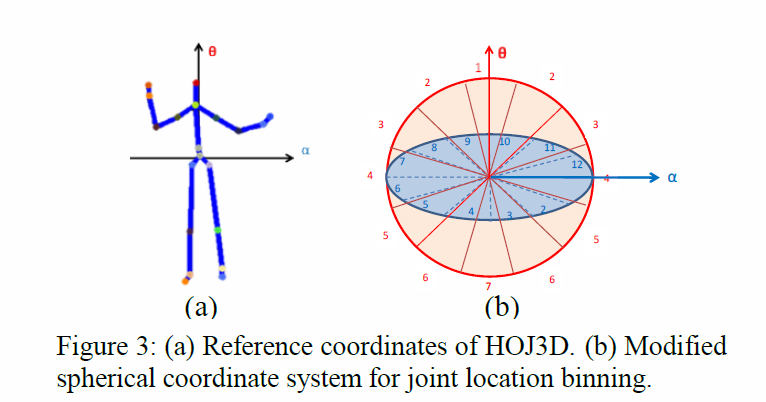
\includegraphics[width=\textwidth]{HOJ3D}
			\end{figure}
			Deze 3D ruimte (figuur 3b) wordt opgesplitst in $n$ partities.
			
			Voor $\theta$: [0, 15], [15, 45], [45, 75], [75, 105] [105, 135], [165, 180]. (7 bins)
			
			Voor $\alpha$: 30 graden voor elke bin, dus 12 bins.
			
			in totaal $7 * 12 = 84$ bins
		
			
			Via deze bolcoördinaten kan elke 3D joint gelokaliseerd worden in een unieke bin 
			\item De 3 joints die gebruikt worden om het bolcoördinatenstelsel te oriënteren staan uiteraard vast. De overige 9 joints worden onderverdeeld in één van de 84 bins. 
			
			\item Om de representatie robust te maken, wordt één enkele joint over verschillende, naburige bins verdeeld (8 buren), op basis van gewichtsfunctie:

			
			\begin{figure}[ht]
				\centering
				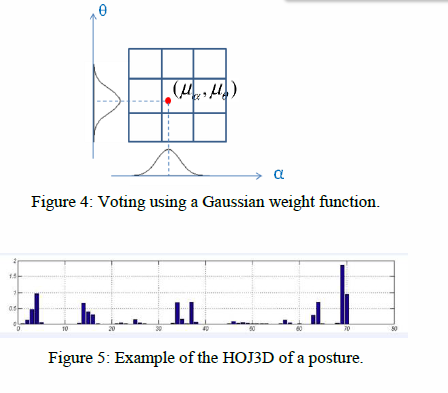
\includegraphics[width=0.5\textwidth]{HO3D_HISTOGRAM}
			\end{figure}
			
			\item Linear discriminant analysis (LDA) wordt toegepast om dominante features eruit deze histogram te halen.
			
			\item Ze stellen voor om kleurenbeelden te combineren met dieptebeelden om algoritmen te ontdekken met beter herkenning
			
			\item Ze beweren sneller te zijn dan bron \cite{action-recognition-based-bag-3d-points}
		\end{itemize}
	\item Bron \cite{action-recognition-based-bag-3d-points} (pre-kinect era)
	\begin{itemize}
		\item Actieherkenning met behulp van reeksen van dieptebeelden
		\item Gaan ervan uit dat efficiënte tracking van skeletbeelden nog niet mogelijk is. (is gepubliceerd zelfde jaar dat Kinect beschikbaar was, 2010)
		\item Hun oplossing is dus niet gebaseerd op het tracken van de skeletbeelden
	\end{itemize}

	\item Bron \cite{Temporal-Action-Detection-with-Structured-Segment-Networks}
	\begin{itemize}
		\item Probleem: output van de actiecategorie EN de start en eind tijd van de actie. 
		\item Ze beweren dat actieherkenning reeds goed opgelost is, maar niet actiedetectie. Hun definities zijn: 
		\begin{itemize}
			\item Actieherkenning: De effectieve actieherkenning indien het systeem weet wanneer hij moet herkennen
			\item Actiedetectie: een langdurige video, waarbij de start en stop van een actie niet gedefinieerd zijn = untrimmed video ( videos waarbij er meerdere acties op hetzelfde moment kunnen voorkomen, alsook een irrelevante achtergrond). {\color{green} sluit heel goed aan op onze masterproef}
		\end{itemize}
		\item Uitdaging in bestaande oplossingen: groot aantal onvolledige actiefragmenten. Voorbeelden:
		\begin{itemize}
			\item Bron \cite{singh2016untrimmed}:
			\begin{itemize}
				\item maakt gebruik van \textbf{untrimmed classificatie}: de top $k = 3$ (bepaalt via cross-validation) labels worden voorspelt door globale video-level features. Daarna worden frame-level binaire classifiers gecombineerd met dynamisch programmeren om de activity proposals (die getrimmed zijn) te genereren. Elke proposal krijgt een label, gebaseerd op de globale label.
			\end{itemize}
				\item Bron \cite{Temporal-Action-Localization-with-Pyramid-of-Score-Distribution-Features}:
			\begin{itemize}
				\item Spreekt over de onzekerheid van het voorkomen van een actie en de moeilijkheid van het gebruik van de continue informatie

				\item Pyramid of Score Distribution Feature (PSDF) om informatie op meerdere resoluties op te vangen
				\item PSDF in combinatie met Recurrent Neural networks bieden performantiewinst in untrimmed videos.
				\item Onbekende parameters: actielabel, actieuitvoering, actiepositie, actielengte
				\item Oplossing? Per frame een verzameling van actielabels toekennen, gebruik makend van huidige frame actie-informatie en inter-frame consistentie = PSDF
	
			\end{itemize}
		
		\end{itemize}
		\item De moeilijkheid is: start, einde en duur van de actie te bepalen.
		\item Hun oplossing is \textbf{Structured Segment Network}:
		\begin{itemize}
			\item input: video
			\item output: actiecategorieën en de tijd wanneer deze voorkomen
			\item Drie stappen:
			\begin{enumerate}
				\item Een "proposal method",  om een verzameling van "temporal proposals", elk met een variërende duur en hun eigen start en eind tijd.  Elke proposal heeft drie stages: \textit{starting, course} en \textit{ending}. 
				\item Voor elke proposal wordt er STPP (structured temporal pyramid pooling) toegepast door (1) de proposal op te splitsen in drie delen; (2) temporal pyramidal representaties te maken voor elk deel; (3) een globale representatie maken voor de hele proposal.
				\item Twee classifiers worden gebruikt: herkennen van de actie en de "volledigheid" van de actie nagaan.
			\end{enumerate}
		\end{itemize}
	\end{itemize}

	\item Bron \cite{Self-Adaptive-Proposal-Model-for-Temporal-Action-Detection-Based-on-Reinforcement-Learning}
	\begin{itemize}
		\item Temporal action detection = moet enerzijds detecteren of al dan niet een actie voorkomt, en anderzijds hoelang deze actie duurt, wat een uitdaging is bij untrimmed videos.
		\item Veel moderne aanpakken gaan als volgt te werk: eerst wordt er klasse-onafhankelijke proposals gegenereerd door 
	\end{itemize}




\end{itemize}
	\chapter{notities}

\section{papers}
\subsubsection{Actieherkenning met skeletdata}


\begin{itemize}



	\item Bron \cite{Zhao2017}
	\begin{itemize}
		\item Probleem: output van de actiecategorie EN de start en eind tijd van de actie. 
		\item Ze beweren dat actieherkenning reeds goed opgelost is, maar niet actiedetectie. Hun definities zijn: 
		\begin{itemize}
			\item Actieherkenning: De effectieve actieherkenning indien het systeem weet wanneer hij moet herkennen
			\item Actiedetectie: een langdurige video, waarbij de start en stop van een actie niet gedefinieerd zijn = untrimmed video ( videos waarbij er meerdere acties op hetzelfde moment kunnen voorkomen, alsook een irrelevante achtergrond). {\color{green} sluit heel goed aan op onze masterproef}
		\end{itemize}
		\item Uitdaging in bestaande oplossingen: groot aantal onvolledige actiefragmenten. Voorbeelden:
		\begin{itemize}
			\item Bron \cite{Singh2016}:
			\begin{itemize}
				\item maakt gebruik van \textbf{untrimmed classificatie}: de top $k = 3$ (bepaalt via cross-validation) labels worden voorspelt door globale video-level features. Daarna worden frame-level binaire classifiers gecombineerd met dynamisch programmeren om de activity proposals (die getrimmed zijn) te genereren. Elke proposal krijgt een label, gebaseerd op de globale label.
			\end{itemize}
				\item Bron \cite{Yuan2016}:
			\begin{itemize}
				\item Spreekt over de onzekerheid van het voorkomen van een actie en de moeilijkheid van het gebruik van de continue informatie

				\item Pyramid of Score Distribution Feature (PSDF) om informatie op meerdere resoluties op te vangen
				\item PSDF in combinatie met Recurrent Neural networks bieden performantiewinst in untrimmed videos.
				\item Onbekende parameters: actielabel, actieuitvoering, actiepositie, actielengte
				\item Oplossing? Per frame een verzameling van actielabels toekennen, gebruik makend van huidige frame actie-informatie en inter-frame consistentie = PSDF
	
			\end{itemize}
		
		\end{itemize}
		\item De moeilijkheid is: start, einde en duur van de actie te bepalen.
		\item Hun oplossing is \textbf{Structured Segment Network}:
		\begin{itemize}
			\item input: video
			\item output: actiecategorieën en de tijd wanneer deze voorkomen
			\item Drie stappen:
			\begin{enumerate}
				\item Een "proposal method",  om een verzameling van "temporal proposals", elk met een variërende duur en hun eigen start en eind tijd.  Elke proposal heeft drie stages: \textit{starting, course} en \textit{ending}. 
				\item Voor elke proposal wordt er STPP (structured temporal pyramid pooling) toegepast door (1) de proposal op te splitsen in drie delen; (2) temporal pyramidal representaties te maken voor elk deel; (3) een globale representatie maken voor de hele proposal.
				\item Twee classifiers worden gebruikt: herkennen van de actie en de "volledigheid" van de actie nagaan.
			\end{enumerate}
		\end{itemize}
	\end{itemize}


	\item Bron \cite{Suolan2017}
	\begin{itemize}
		\item Depth-based action recognition.
		\item \textit{key frames} worden geproduceerd uit skeletsequenties door gebruik te maken van de joints als \textbf{spatial-temporal interest points (STIPs)}. Deze worden gemapt in een dieptesequentie om een actie sequentie te representeren. De contour van de persoon wordt per frame bepaald. Op basis van deze contour en de tijd worden features opgehaald. Als classifier gebruiken ze een \textit{extreme learning machine}
		\item Voordeel van key frames: ze bevatten de meest informatieve frames. Twee methodieken om de key frames op te halen:
		\begin{enumerate}
			\item \textbf{Interframe difference}: een nieuwe key-frame wordt gekozen als het verschil tussen twee frames een bepaald threshold overschrijft.
			\item \textbf{Clustering}: groeperen van frames die op elkaar lijken op basis van low-level features. Uit die groep wordt dan de keyframe genomen, die het dichtst bij het centrum van dat cluster ligt.
		\end{enumerate}
		\item Zij gebruiken het 'opgenomen verschil': Een positie van een joint $P_{i,j}$ met $i$ het frame index en $j$ de joint index, kan gelijkgesteld worden als  $P_{i, j} = {x_{i, j}, y_{i, j}, z_{i, j}}$
		
		Het opgenomen verschil is dan:
		
		$$D_i = \sum_{j = 1}^{n} || P_{i, j} - P_{i - 1, j}||^2$$
		met $||\cdot||$ de euclidische afstand en $n$ het aantal joints.
		
		\item key frames worden dan gekozen op basis van maximum of minimum $D_i$ binnen een sliding window. Een probleem: $D_i$ is vrij laag voor de eerste en laatste aantal frames. De key frames worden dus eerder gecentraliseerd en kan de sequentie niet accuraat bepaalt worden. Stapsgewijze oplossing:
		\begin{enumerate}
			\item Voor een video met $N$ frames: neem de som van $D_i$ van $i = 2$ tot $i = N$:
			$$D_N = \sum_{i = 2}^{N}D_i$$
			\item Bepaal een aantal key frames $K$ en bereken het gemiddelde van incrementen:
			
			$$D_{avg} = D_N / K$$
			
			\item Voor $i = 2$ tot $i = L$ wordt het verschil berekent:
			
			$$W_L = D_L - k * D_{avg}, k \in K$$
			
			zodat er een verzameling ${W_L}$ is. Het minimum van deze set wordt de key frame.
		\end{enumerate}
		\item Features op basis van contour
		\item Actieherkenning met neurale netwerken (EXTREME LEARNING)
		\item \textbf{Samenvatting:}
		\begin{itemize}
			\item Actionherkenningsmethode voor kinect.
			\item Features op basis van menselijke contour van een keyframe uit een dieptebeeld. Als constraint is er het temporaal verschil.
			\item 'multi-hidden layer extreme learning machine' voor classificatie
		
		\end{itemize}
		
	\end{itemize}
\end{itemize}




\section{Machine learning}
\subsection{Features}
\begin{itemize}
	\item Een \textbf{feature} is een individueel, meetbare eigenschap of karakteristiek van een object dat geobserveerd wordt.
	\item Eigenschappen:
	\begin{itemize}
		\item Informatief: de informatiewinst van de feature moet hoog zijn
		\item Discriminative: op basis van de feature moet het eenvoudig zijn om het onderscheid te maken tussen de verschillende klassen
		\item Onafhankelijk: De feature op zich mag van geen andere feature of meetwaarde van dezelfde feature afhangen.


	\end{itemize}
	\item Een \textbf{sparse feature discriptor} heeft een variabel aantal features. Een \textbf{dense feature descriptor} heeft een vast aantal features.
	\item \textbf{Feature extraction} ($\equiv$ dimensionality reduction) is het verzamelen van features uit ruwe data zodat deze kunnen gebruikt worden als feature vector bij een classifier. 
	\item Een \textbf{feature vector} is een $n$-dimensionale vector van \underline{numerieke} features.
	\item De \textbf{feature space} ($\equiv$ vectorruimte) beschrijft de ruimte waarin de features zich bevinden. (bv 3 verschillende features = $\mathcal{R}^3$)
	\item \textbf{Feature construction} is het maken van nieuwe features op basis van reeds bestaande features. De mapping is een functie $\phi$, van $\mathcal{R}^n$ naar $\mathcal{R}^{n + 1}$, met $f$ de geconstrueerde feature op basis van bestaande features, bv $f = x_1/x_2$.
	
	$$\phi(x_1, x_2, ..., x_n) = (x_1, x_2, ... x_n, f)$$

\end{itemize}
\subsection{Classifier}
\begin{itemize}
	\item Identificeren tot welke klasse een \underline{nieuwe} observatie behoort, gebaseerd op een training set waarvan de klassen wel gekend zijn.
	\item \textbf{Lineaire classifiers} geven aan elke klasse $k$ een score op basis van de combinatie van de feature vector met een gewichtenvector met het scalair product.  De gekozen klasse is dan die met de hoogste score. Eenvoudiger geschreven:	
	$$
	score(X_i, k) = \beta_k \cdot X_i
	$$
	\begin{itemize}
		\item $X_i$ = de feature vector voor instantie $i$
		\item $\beta_k$ = de gewichtenvector voor klasse $k$
	\end{itemize}
	\item \todo{later onderzoeken}
	\item \textbf{Support Vector machines}
	\item \textbf{Random forests}
	\item \textbf{Boosting}
\end{itemize}




\subsection{Hidden Markov Model}
\label{sec:hidden_markov_model}
Bron \cite{Ramage2007}
\subsubsection{Markov model}

\begin{itemize}
	\item Markov process = stochastisch process met volgende eigenschappen:
	\begin{itemize}
		\item Het aantal toestanden $S = \{s_1, s_2, ... s_{|S|}\}$ is eindig.
		\item Observatie van een sequentie over de tijd $\textbf{z} \in S^T$
		
		Voorbeeld: 
		
		$S = \{sun, cloud, rain\}$ met $|S| = 3$ en $\textbf{z} = \{z_1=S_{sun},z_2=S_{cloud},z_3=S_{cloud},z_4=S_{rain},z_5=S_{cloud}\}$ met $T = 5$.
		\item Markov Assumpties:
		\begin{enumerate}
			\item Een toestand is enkel afhankelijk van de vorige toestand (\textbf{Markov Property}).
			
			$$P(z_t | z_{t - 1},z_{t-2}, ..., z_1) = P(z_t|z_{t-1})$$
			\item De waarschijnlijk is constant in de tijd
			
			$$P(z_t|z_{t - 1}) = P(z_2|z_1); t \in 2 ...T$$
		\end{enumerate}
		\item Beginstaat $z_0 \equiv s_0$.
		\item Transitiematrix $A \in \mathbb{R}^{(|S| + 1)\times(|S| + 1)}$, met $A_{ij} = P(i \rightarrow j)$, :
		
		$$A = \begin{matrix}
		     & s_0 & s_{sun} & s_{cloud} & s_{rain} \\
		 s_0 & 0 & .33 & .33 & .33 \\
		 s_{sun} & 0 & .8 & .1 & .1 \\
		 s_{cloud} & 0 & .2 & .6 & .2 \\
		 s_{rain} & 0 & .1 & .2 & .7 \\
		\end{matrix}$$
	\end{itemize}

\end{itemize}

\begin{itemize}
	\item Twee vragen die een markov model kunnen oplossen:
	\begin{enumerate}
		\item Wat is de kans op een bepaalde toestandenvector $\textbf{z}$?

				$$	P(\textbf{z})  = \prod_{t=1}^{T} A_{z_{t-1}z_t}$$

			Stel $\textbf{z} = \{z_1=S_{sun},z_2=S_{cloud},z_3=S_{rain},z_4=S_{rain},z_5=S_{cloud}\}$ dan is $P(\textbf{z}) = 0.33 \times 0.1 \times 0.2 \times 0.7 \times 0.2 $
		\item Gegeven $\textbf{z}$, hoe worden best de parameters van $A$ benaderd zodat de kans op $\textbf{z}$ maximaal is.
		$$A_{ij} = \frac{\sum_{t=1}^{T} \{z_{t-1} = s_i \wedge z_t = s_j\}}{\sum_{t=1}^{T} \{z_{t-1} = s_i\}}$$
		
		De maximale kans om van staat $i$ naar $j$ te gaan is het aantal transities van $i$ naar $j$ gedeeld door het totaal aantal keer dat we in $i$ zitten. Met andere woorden: Hoeveel \% zaten we in $i$ als we van $j$ komen.
	\end{enumerate}
\end{itemize}

\subsubsection{Hidden Markov Model}
\begin{itemize}
	\item \gls{ac:hmm} = Veronderstelt een markov process met verborgen toestanden
	\item Bij een HMM: de staat is niet zichtbaar, maar de output is wel zichtbaar.
	\item Formeel:
	\begin{itemize}
		\item Sequentie van geobserveerde outputs $x = \{x_1, x_2, ..., x_T\}$  uit een alfabet $V = \{v_1, v_2, ..., v_{|V|}\}$
		\item Er is ook een sequentie van staten $z =\{z_1, z_2, ... z_T\}$ uit een alfabet $S = \{s_1, s_2, ... s_{|S|}\}$, maar deze zijn \underline{niet zichtbaar}.
		\item Transitiematrix $A_{ij}$ wel bekend.
		\item Kans dat een bepaalde output gegenereerd wordt in functie van de verborgen toestanden:
		
		$$P(x_t = v_k|z_t = s_j) = P(x_t = v_k | x_1, ..., x_T, z_1, ..., z_T) = B_{jk}$$
		
		Matrix $B$ geeft de waarschijnlijkheid dat een verborgen toestand $s_j$ de output $v_k$ teruggeeft.
	\end{itemize}
	\item Vaak voorkomende problemen die opgelost kunnen worden met HMM:
	\begin{itemize}
		\item Gegeven de parameters en geobserveerde data, benader de optimale sequentie van verborgen toestanden.
		\item Gegeven de parameters en geobserveerde data, bereken de kans op die data. $\rightarrow$ Wordt het 'decoding' probleem (\textbf{Viterbi Algoritme}) genoemd en wordt gebruikt bij continue actieherkenning.
		\item Gegeven de geobserveerde data, benader de parameters van $A$ en $B$.
	\end{itemize}
	\item Het \textbf{decoding probleem}: \url{http://jedlik.phy.bme.hu/~gerjanos/HMM/node8.html}
	\begin{itemize}
		\item Zoek de meest waarschijnlijke reeks van toestanden $\textbf{z} \in S^T$ voor een verzameling van observaties $\textbf{x} \in V^T$.
		
		\item Hoe 'meest waarschijnlijke toestandensequentie' definiëren. Een mogelijke manier is om de meest waarschijnlijke staat $s_t$ voor $x_t$ te berekenen, en alle $q_t$ dier daar aan voldoen te concateneren.
		Andere manier is \textbf{Viterbi algoritme} die de hele toestandensequentie met de grootste waarschijnlijkheid teruggeeft.
		
		\item Hulpvariabele:
		
		$$\delta_t(i) = \max_{\substack{q_1, q_2, ... q_{t-1}}} p\{q_1, q_2, ... q_{t - 1}, q_t = i, o_1, o_2, ... o_{t - 1} | \lambda \}$$
		
		die de hoogste kans beschrijft dat een partiele observatie en toestandensequentie tot $t = t$ kan hebben, wanneer de huidige staat $i$ is.
	\end{itemize}
\end{itemize}



%	\chapter{Conclusie}
\label{ch:Conclusie}
	
	\printglossaries
	

%	\listoffigures
%	\listoftables
	
	
	\bibliographystyle{IEEEtran}
	\bibliography{bib/library}
	
\end{document}